%
% Modified by Megan Patnott
% Last Change: Jan 18, 2013
%
%%%%%%%%%%%%%%%%%%%%%%%%%%%%%%%%%%%%%%%%%%%%%%%%%%%%%%%%%%%%%%%%%%%%%%%%
%
% Modified by Bryce Frentz
% Last Change: 2018
%
%%%%%%%%%%%%%%%%%%%%%%%%%%%%%%%%%%%%%%%%%%%%%%%%%%%%%%%%%%%%%%%%%%%%%%%%
%
% Sample Notre Dame Thesis/Dissertation
% Using Donald Peterson's ndthesis classfile
%
% Written by Jeff Squyres and Don Peterson
%
% Provided by the Information Technology Committee of
%   the Graduate Student Union
%   http://www.gsu.nd.edu/
%
% Nothing in this document is serious except the format.  :-)
%
% If you have any suggestions, comments, questions, please send e-mail
% to: ndthesis@gsu.nd.edu
%
%%%%%%%%%%%%%%%%%%%%%%%%%%%%%%%%%%%%%%%%%%%%%%%%%%%%%%%%%%%%%%%%%%%%%%%%

%
% Chapter 2
%

\chapter{Experimental setup and procedures}
\label{chap: experiment}

\section{Introduction}

This chapter is included to highlight some techniques and equipment commonly used in low-energy nuclear physics, with an emphasis on those used in this work. The discussion will be presented from the lens of the general to the specific, introducing general concepts for beam production and transport, acceleration systems, and radiation detection. Following the discussion of the scientific principles, I will detail the specifics of the equipment employed in this collective work. To that end, I will also highlight differences between the facilities and techniques employed when compared to common equipment for nuclear physics experiments


\section{Experimental Equipment}
\label{sec: equipment}



\subsection{Accelerators}
\label{sec: accelerators}

First and foremost, low-energy nuclear physics (generally understood to be the regime in which incident kinetic energies for reactions are below 1 GeV, often even as low as sub-MeV) requires particle acceleration systems in order to bring beams and targets together. The most common techniques for accelerating ions are 1) to use strong electrostatic fields for a straight-line acceleration, such as in the Van de Graaff accelerator, or 2)  by using a combination of electric and magnetic fields to accelerate the particles in cyclotron motion, aptly named a cyclotron. Van de Graaff accelerators are the most prominent of all accelerators, though, and are the type used in this work. 

The basic idea of a Van de Graaff accelerator is shown in Fig. \ref{fig: vdg principles}. The governing principle is that a beam of ions produced in an ion source (Section \ref{sec: ion sources}) are manipulated by additional electromagnetic elements (Section \ref{sec: beamline}) into an area of high electric potential. This high voltage is produced and maintained by continuously transporting positive charge from ground to a Faraday cage with a field free interior (referred to as the terminal, with voltage $V_{T}$). The positively charged ions, being in close proximity to the positively charged terminal feel a repulsive force, accelerating the ions out of the terminal and through the machine. Upon exiting the accelerator, the ions have energy

\begin{equation}
E_{ion} = qV_{T} = \dfrac{1}{2} m_{ion} v_{ion}^{2}
\label{eqn: accelerator}
\end{equation}

\noindent where $V_{T}$ again is the terminal voltage and $q$ is the charge state of the ion going through the accelerator, $m_{ion}$ is the mass of the ion, and $v_{ion}$ is the ion's velocity. When the terminal voltage is in MV, the beam energy is then provided in MeV. Specifically for the 5U accelerator, though, Equation \ref{eqn: accelerator} must be modified with an additional term. Inside the ion source, there is an electrostatic extractor, which transports the beam of ions out of the terminal and into the acceleration tube. With this correction, the beam energy for the 5U is given as

\begin{equation}
E_{ion} = q(V_{extractor} + V_{T}).
\end{equation}

\begin{figure}
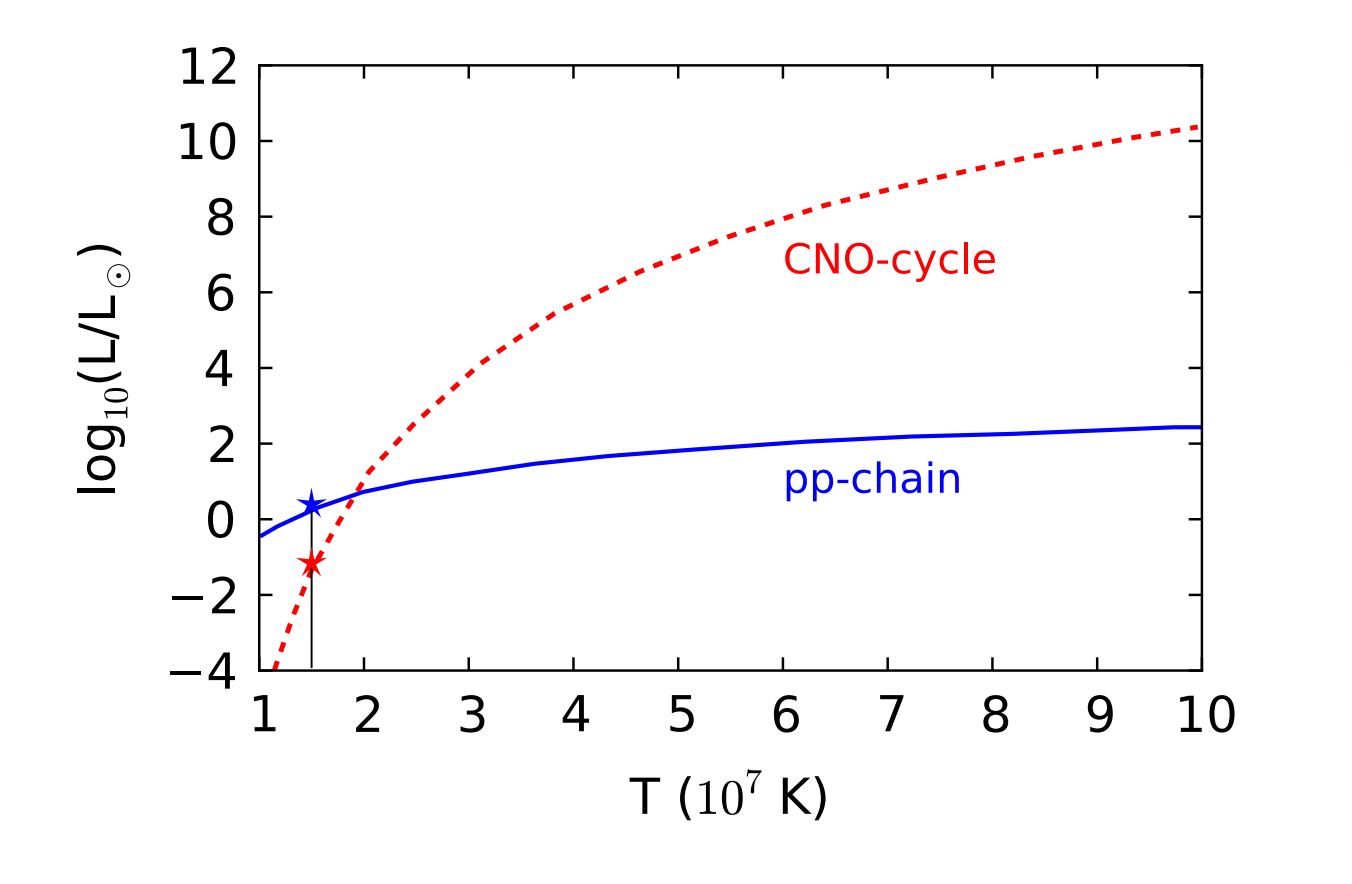
\includegraphics[width=\linewidth]{figures/energyProduction.png}
\label{fig: vdg principles}
\caption{A diagram of a Van de Graaff accelerator \cite{RolfsBook}. The charge transportation in this figure is shown with a belt, like the JN accelerator model at CASPAR, while the 5U accelerator at the NSL uses a Pelletron chain. }
\end{figure}

The charge is delivered to the terminal via a mechanical delivery system. The 5U Sta. Ana accelerator at the NSL uses four Pelletron chains cite{Herb1974}, each with its own power supply, while the JN Van de Graaff accelerator at CASPAR utilizes a rotating belt. In either case, the entire charging system is contained inside of a pressurized tank of insulating gas, SF$_{6}$ for the 5U and CO$_2$ for the JN, reducing the chance of a terminal discharge to ground from dielectric breakdown. This is not the only element to ensure the operational stability of the machine. The charging systems supply charge continuously to the terminal. However, charge is always being removed from the terminal via three primary pathways: 1) the beam of ions passing through the accelerator, 2) the resistive column, and 3) the corona system. In order to maintain stability, the currents that pass through these systems must always be in balance according to Kirchoff's Rule,

\begin{equation}
I_{chains} = I_{beam} + I_{column} + I_{corona}.
\end{equation}

\noindent The column is actually a series of equipotential hoops connected by equal resistors. Each conducting hoop provides a small step down in voltage from the terminal, ensuring that the beam of ions feel a smooth potential gradient throughout their acceleration. These can be seen in Fig. \ref{fig: column}, showing an interior view of Sta. Ana accelerator tank. 


\begin{figure}
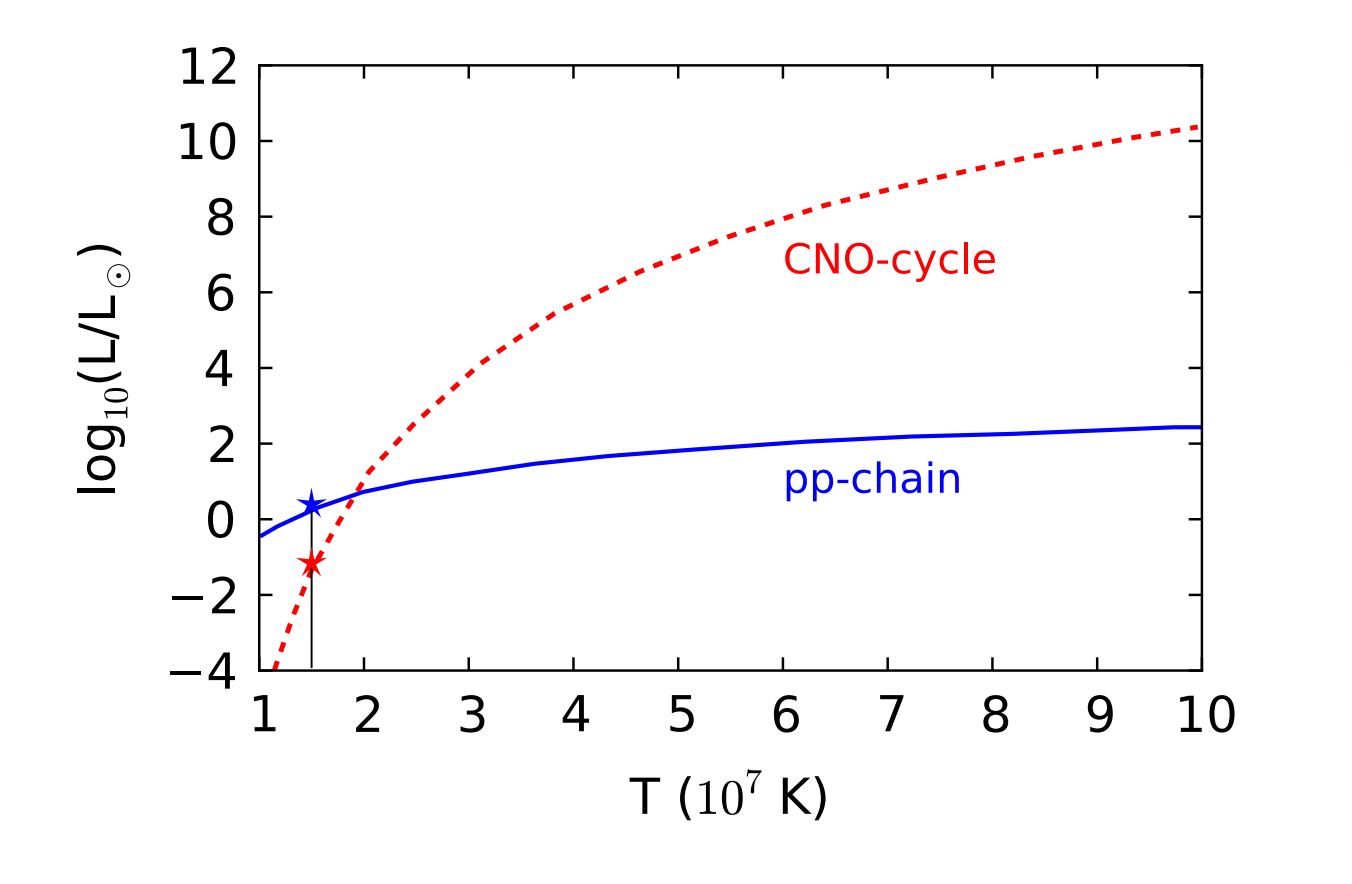
\includegraphics[width=\linewidth]{figures/energyProduction.png}
\label{fig: column}
\caption{View inside the Sta. Ana accelerator tank, showing the equipotential hoops as part of the column.}
\end{figure}


The corona system is the real workhorse maintaining the stability of the accelerator's charging systems. As small irregularities can be present between different links in the Pelletron chains or the belt itself, the corona system is responsible for precise second-by-second compensation. The mechanical part of the system consists of an arm with sharp metal points on the end which can be moved towards and away from the terminal to draw away current. On the back end, however, it also is controlled by a voltage feedback system to adjust the current draw, keeping the terminal at a constant voltage. The feedback for the system is provided either by an external reference through a generating voltmeter or from the beam itself as it passes through an analyzing dipole magnet at the exit of the accelerator. As the beam passes through the magnet it will pass through a set of slits. If $V_{T}$ changes slightly, the energy of the beam will subsequently change, impacting the balance of the beam on the exit slits. This change in current will be fed back to the corona system, which in turn will compensate by changing the charge delivered to the terminal in order to maintain the slit balance. With this, $V_{T}$ can be kept incredibly steady, within roughly 1 kV for every MV on the terminal. This is the biggest advantage of a Van de Graaff accelerator over a cyclotron. Intrinsically, this acceleration system makes nuclear experiments possible through monoenergetic beams. 


\subsection{Ion sources}
\label{sec: ion sources}

A key item for the successful operation of any accelerator is the ion source, which produces the beams of charged particles used in experiments. Generating such beams is not a trivial task and, as such, many methods have been developed for achieving this. The two types relevant to this work, however, are the Electron-Cyclotron Resonance (ECR) ion source, used in the Sta. Ana accelerator at the NSL, and the radio frequency (RF) ion source, utilized in the JN accelerator at CASPAR.  Both systems are housed within their respective accelerator terminals, which acts as a Faraday cage and shields the internal components from external fields.


ECR

RF

\subsection{Beam transport}
\label{sec: beamline}


Why vaccuum and how?

Cold trap

Magnets for steering, focusing, analyzing


\subsection{Radiation detection}
\label{sec: detectors}



types

photon interactions with matter

HPGe


\section{The CASPAR facility and cross-section measurements}
\label{sec: cs experiment}



This set of data was taken over the course of five* separate experiments. The first occurred at the University of Notre Dame's Nuclear Science Laboratory (NSL) in January of 2018 and covered the proton energy range of E$_{p}$ = 800 - 1200 keV. The experiment was then continued at the Compact Accelerator System for Performing Nuclear Astrophysics (CASPAR) facility at the Sanford Underground Research Facility located in Lead, South Dakota in three increments: February 2018, May 2018, and August / September 2018. These measurements covered the energy range from E$_{p}$ = 270 - 1200 keV, in order to measure the $^{14}$N$\left( p,\gamma \right) ^{15}$O reaction cross-section to compare the performance of the CASPAR facility to an above-ground laboratory. Finally, in MONTH TIME DATE THING, the final experiment was completed at the NSL, focusing on obtaining the lifetime of the 6793 keV state in $^{15}$O.

Reiterate why we went underground and its advantages
Background comparison

Describe experiment (PJ)


\section{Lifetime measurement}
\label{sec: lifetime experiment}

\subsection{The Doppler-Shift Attsenuation Method}
\label{sec: DSAM}

Copy and paste from chapter 1

\subsection{Target production}
\label{sec: implantation}

Why Implantation
Seuthe
How did we produce them and why

\subsection{Measurement at Notre Dame}

How did we do it
Highlight similarities and differences to previous measurements.




% % uncomment the following lines,
% if using chapter-wise bibliography
%
% \bibliographystyle{ndnatbib}
% \bibliography{example}
